
The variations mentioned in the previous section were tried and the analysis of the perfromance of KNN classifier is presented in this section.
\subsection{Classifier Performance for Iris Dataset}
	\textbf{Classifier 1}
	\begin{itemize}
		\item Preprocessing - Simple Scaling
		\item Proximity Metric - Euclidean Distance
		\item Voting - Inverse Distance Weighted Voting
	\end{itemize}
	The confusion matrix for k = 5 is given in Fig: ?
	\begin{figure}[h]
		\label{fig:iris_k=5}
		\caption{Confusion Matrix k = 5 (Datset:Iris Classifier:1)}
		\centering
		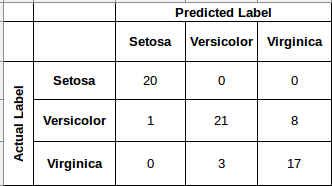
\includegraphics[width=0.4\textwidth]{images/iris_k=5.png}
	\end{figure}
	From the analysis in the previous assignment, we know that the setosa class was distinctly separated from the other two classes. The effect of this can be seen in the confusion matrix. The KNN classifier was able to classify all instances of setosa correctly. Also, there was only 1 false positive for setosa. On the other hand, versicolor and virginica had significant overlap. The algorithm did a good job on them too. Although, roughly 33\% of Versicolor were falsely classified as Virginica. Overall the accuracy of this classfier was 82\% \\
	
	\textbf{Classifier 2}
	\begin{itemize}
		\item Preprocessing - Simple Scaling (same as before)
		\item Proximity Metric - Cosine Similarity
		\item Voting - Inverse Distance Weighted Voting (same as before)
	\end{itemize}
	The confusion matrix for $k = 5$ is given in Fig: ??.
	\begin{figure}[h]
		\label{fig:iris_consine_k=5}
		\caption{Confusion Matrix k = 5 (Datset:Iris Classifier:2)}
		\centering
		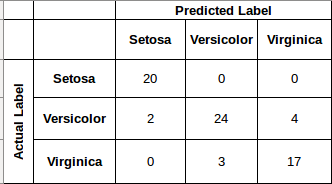
\includegraphics[width=0.4\textwidth]{images/iris_cosine_k=5.png}
	\end{figure}
	This classifier performed better than the previous one. The accuracy increased to 87\%, by simply by using cosine similarity instead of euclidean similarity. Here to setosa was much more easily distinguised as compared to the other two classes, although the false positives in setosa increased increased by small amount.\\

\subsection{Classifier Performance for Income Dataset}
For binary income dataset, the classifier had to be optimized over two parameters had to be optimized - the number of nearest neighbours $k$ and threshold for making the prediction. \\
To optimum $k$ for the classifier would be the $k$ for which the ``Area Under the Roc Curve" is maximized. To find the optimum $k$, the roc graphs were computed over the test set for $k$'s ranging from 1 to 100. It was expected that the area would increase with $k$, peak and then plateau out. The $k$ at the peak would then be optimum.\\
For a picking the optmium threshold, we maximized the accuracy of the classifier. To determine the highest accuracy, the threshold was varied keeping the $k$ was fixed. The threshold for which the accuracy is maximum was taken to be the optimum threshold.

\textbf{Classifier 1}
	\begin{itemize}
		\item Preprocessing - Simple Scaling
		\item Proximity Metric - Euclidean Distance
		\item Voting - Inverse Distance Weighted Voting
	\end{itemize}
	For this classifier the Area under ROC reaches maximum at $k = 38$. In Fig. ?? four ROC curves have been plotted. The ROC curve for $k=38$ has the most area underneath it, although it is surpassed at few points by other ROC curves. The accuracy for $k=38$ is plotted as a function of $threshold$. It increase monotonically as $threshold$ increases and is maximum for $threshold=1$ (point not on the curve). This is beacuse of the highly skewed class ratio, the highest accuracy is obtained when all records are classified as negative. This is clearly not a $threshold$ to pick. However, if we give more weightage to true positives, the Accuracy Vs Threshold Curve might for values less than one, giving a more reasonable classifier. \\
	\begin{figure}[h]
		\label{fig:classifier1_auc}
		\caption{Plot of Area Under the Roc curve for different values of k for Income Classifier 1. Maxima is achieved at k = 38}
		\centering
		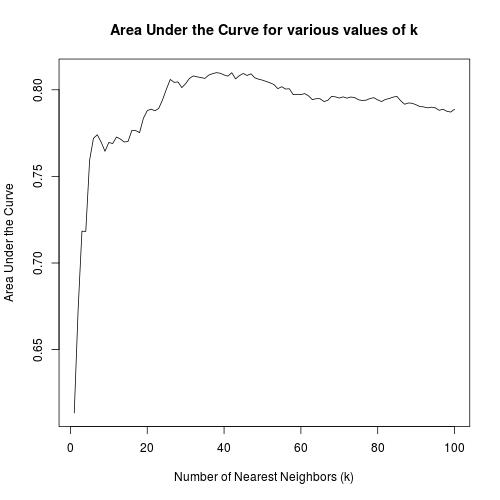
\includegraphics[width=0.3\textwidth]{images/income_classifier1/auc.jpg}
	\end{figure}	
	\begin{figure}
		\label{fig:classifier1_roc}
		\caption{ROC curves for different values of k for Income Classifier 1}
		\centering
		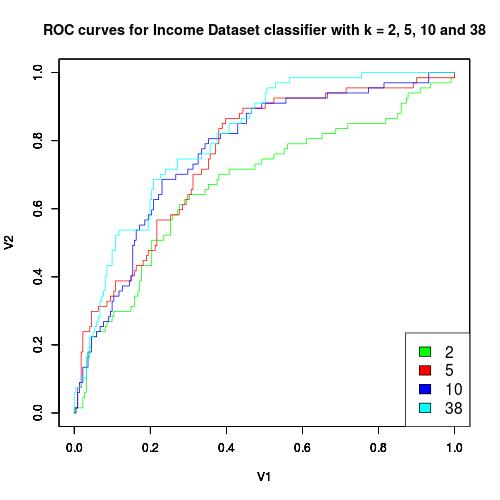
\includegraphics[width=0.3\textwidth]{images/income_classifier1/roc.jpg}
	\end{figure}
	\begin{figure}
		\label{fig:classifier1_accuracy}
		\caption{Plot of Accuracy Vs Threshold Values for k = 38}
		\centering
		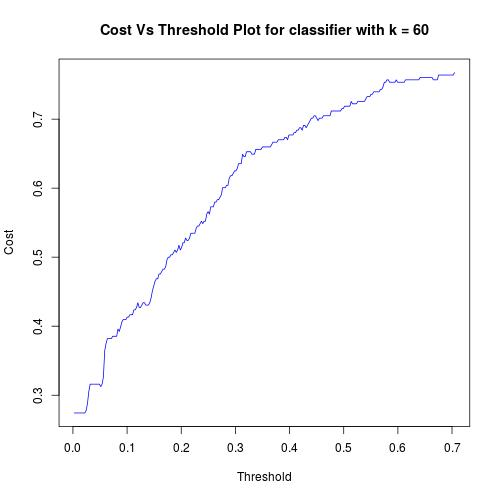
\includegraphics[width=0.3\textwidth]{images/income_classifier1/accuracy.jpg}
	\end{figure}	
	
\textbf{Classifier 2}
	\begin{itemize}
		\item Preprocessing - Simple Scaling
		\item Proximity Metric - Cosine Similarity
		\item Voting - Inverse Distance Weighted Voting
	\end{itemize}
	The Iris dataset should a good improvement when the proximity metric was changed from eulidean distance to cosine similarity. However, the same is not observed in income dataset. For this classifier the ``area under the curve" reaches its maximum at k=38. Fig. ?? contains the plot for the AUC. Four different ROCs have been plotted in Fig. ??. The trend in AUC and ROC is similar to what was observed in previous classifier. The best accuracy too is obtained for $threshold=1$. The false positive rate increase way to fast in comparison to the true positive rate.\\
	\begin{figure}[h]
		\label{fig:classifier2_auc}
		\caption{Plot of Area Under the Roc curve for different values of k for Income Classifier 2. Maxima is achieved at k = 36}
		\centering
		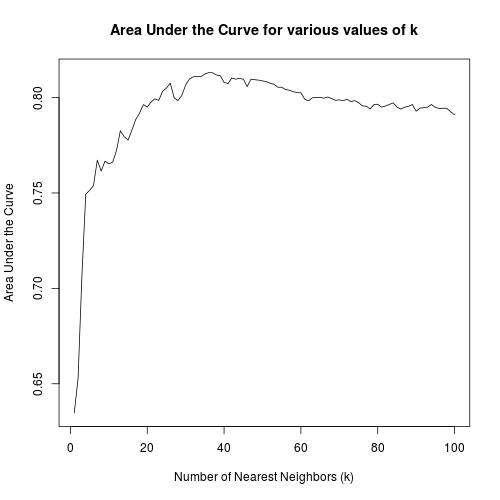
\includegraphics[width=0.3\textwidth]{images/income_classifier2/auc.jpg}
	\end{figure}	
	\begin{figure}
		\label{fig:classifier2_roc}
		\caption{ROC curves for different values of k for Income Classifier 2}
		\centering
		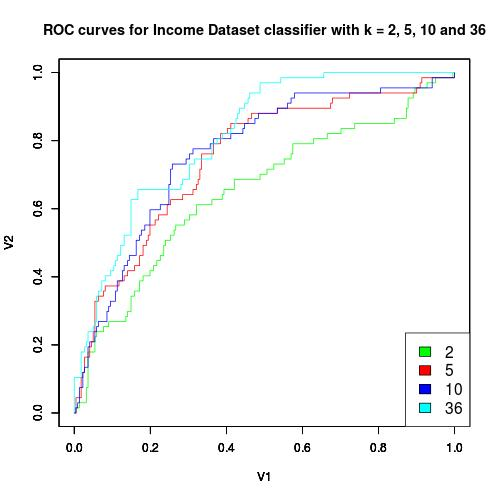
\includegraphics[width=0.3\textwidth]{images/income_classifier2/roc.jpg}
	\end{figure}
	\begin{figure}
		\label{fig:classifier2_accuracy}
		\caption{Plot of Accuracy Vs Threshold Values for k = 36}
		\centering
		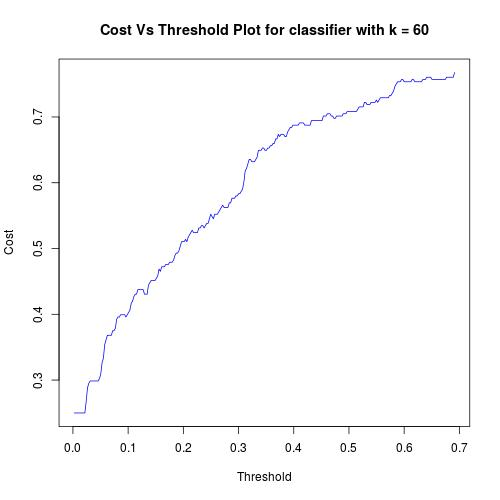
\includegraphics[width=0.3\textwidth]{images/income_classifier2/accuracy.jpg}
	\end{figure}
	
\textbf{Classifier 3} - Best Performance
	\begin{itemize}
		\item Preprocessing - Simple Scaling with Binning
		\item Proximity Metric - Cosine Similarity
		\item Voting - Inverse Distance Weighted Voting
	\end{itemize}
	Based on the previous performance of the previous two classfiers, it was felt that the attributes should be preprocessed such that the similar record have similar values. In that spirit, many categories were merged. For e.g - There were 26 native countries, with 12 having only one record. Each of these records belonged to the same class. The records would be 1 unit apart if simple dissimilarity is computed. But for this classifier all these records were bunched together in a single category and hence bringing them closer.\\
	These preprocessing did have a small postive effect. The maximum area under the curve incrased by 5\% (Fig. ??). The ROC for optimium $k$ also reaches a saturation at lower FPR as compared to Classfier 1 or 2. However, the the optimium $threshold$ is still $1.0$.\\
	\begin{figure}[h]
		\label{fig:classifier3_auc}
		\caption{Plot of Area Under the Roc curve for different values of k for Income Classifier 3. Accuracy keeps increaing beyond hundred}
		\centering
		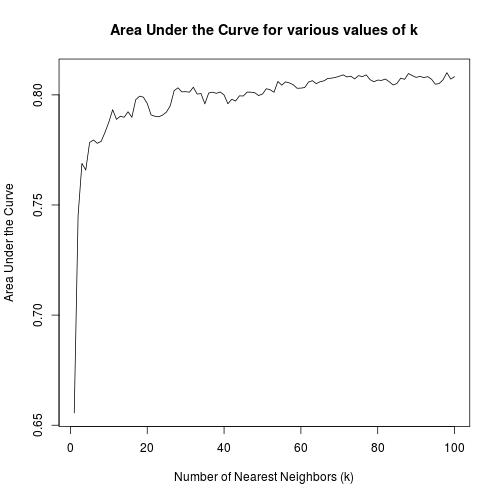
\includegraphics[width=0.3\textwidth]{images/income_classifier3/auc.jpg}
	\end{figure}	
	\begin{figure}
		\label{fig:classifier1_roc}
		\caption{ROC curves for different values of k for Income Classifier 3}
		\centering
		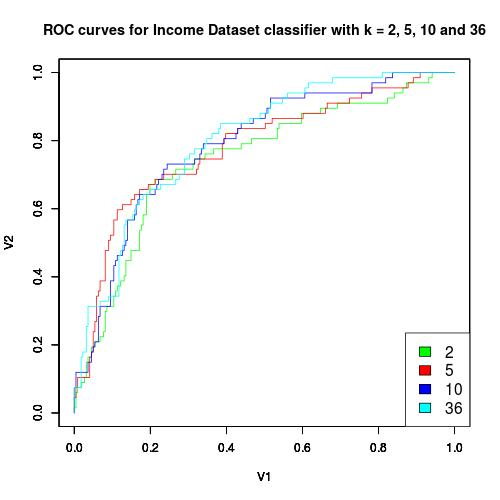
\includegraphics[width=0.3\textwidth]{images/income_classifier3/roc.jpg}
	\end{figure}
	\begin{figure}
		\label{fig:classifier3_accuracy}
		\caption{Plot of Accuracy Vs Threshold Values for k = 40}
		\centering
		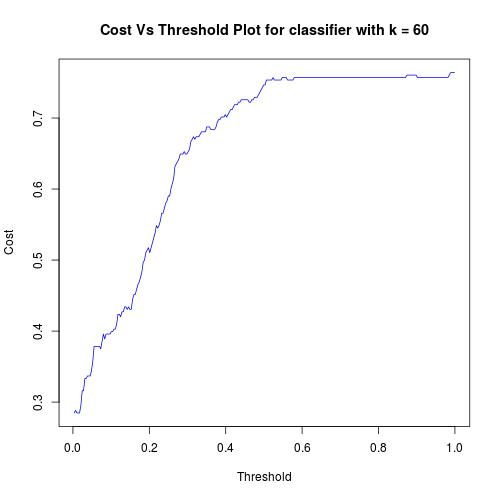
\includegraphics[width=0.3\textwidth]{images/income_classifier3/accuracy.jpg}
	\end{figure}
	
\subsection{Answer to Select Homework Questions}
A,B) The Precision, Recall and F-Measure  are plotted in Fig. ??\\
\begin{figure}
	\label{fig:confusion}
	\caption{Precision, Recall and F-Measure for Classifier 3 of Income Data test set}
	\centering
	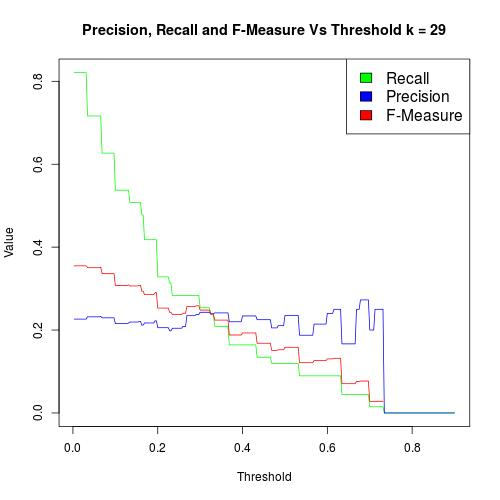
\includegraphics[width=0.3\textwidth]{images/prf.jpg}
\end{figure}
D) There was effect of proximity measure. It was more pronuced on Iris than Income dataset.\\
E) To understand the effect of $k$ on the classifier the AUC can be observed. As mentioned earlier in this report the classfier becomes better for a while, then it peaks and then plateaus. (Fig. ??)\\
F) The third varion in Section. ?? was added becuase the algorithm was not working well with data.
